% himcm-paper.tex 

\title{Epi-Dealing with Epidemics}
\date{November 2014}
\author{Team \#\#\#\#}

\documentclass[12pt]{article}
\usepackage{graphicx}
\usepackage{fancyhdr}
\usepackage{lastpage}
\usepackage{amsmath}
\usepackage{mathtools}
\usepackage[total={6in,8in}]{geometry}

\pagestyle{fancy}

\begin{document}
\lhead{Team 4637}
\rhead{Page \thepage \hspace{1pt} of \pageref{LastPage}}
\cfoot{}

\section{Summary}
Faced with the challenge of analyzing an unknown disease and determining an appropriate course of actions, our team developed a model to determine the behavior of the disease and simulate its spread in the village. To add accuracy to our model, given relatively little information, we ran the model countless times with different parameters in an attempt to generalize the disease’s behavior.

We first looked toward the SIR model as the foundation of our simulation. We split the people of the village into types: Susceptible, Infected, Recovered, as well as Dead. We also accounted for the potential latent period of infection. Next we looked at the Rumor Spreading Model for insight. We had assumed the disease was spread through human interaction rather than the use of vectors or other means. Therefore, we compared the spreading of a rumor to the spreading of a disease, as both require human interaction and involve spreaders and receivers. We manipulated the formula of rumor spreading to fit our model of the spreading of infection, and determined the probability of a particular infected person infecting a susceptible person.

From these two models, we coded using Java our own model that simulated the spread of infection. We used the given values of infected and susceptible to start with and allowed the members of the village to interact each day. However, since we did not know many values crucial to determining the behavior of spread, we set them as modifiable variables, seeing what would happen under different assumed conditions. We ran this program until the number of infected people reached 0; in other words, the disease is exterminated.

We analyzed the data we received to classify the type and severity of the disease, and whether or not the epidemic was contained. We concluded that this disease followed the behavior of a point source outbreak, and the epidemic was quickly contained. From further analysis of our data, we also devised recommendations to prevent the spread of this disease: namely, preventing contact with infected individuals as well as preventing contact between this village and any other village.

When more information was learned about the particular disease, we were able to create a more accurate model. We were also able to take into account different situations--including the spread of the disease to other municipalities. However, we have faith that the nature of the disease and the consideration of our recommendations will prevent the continued spread of this dangerous disease.

\newpage
\begin{center}
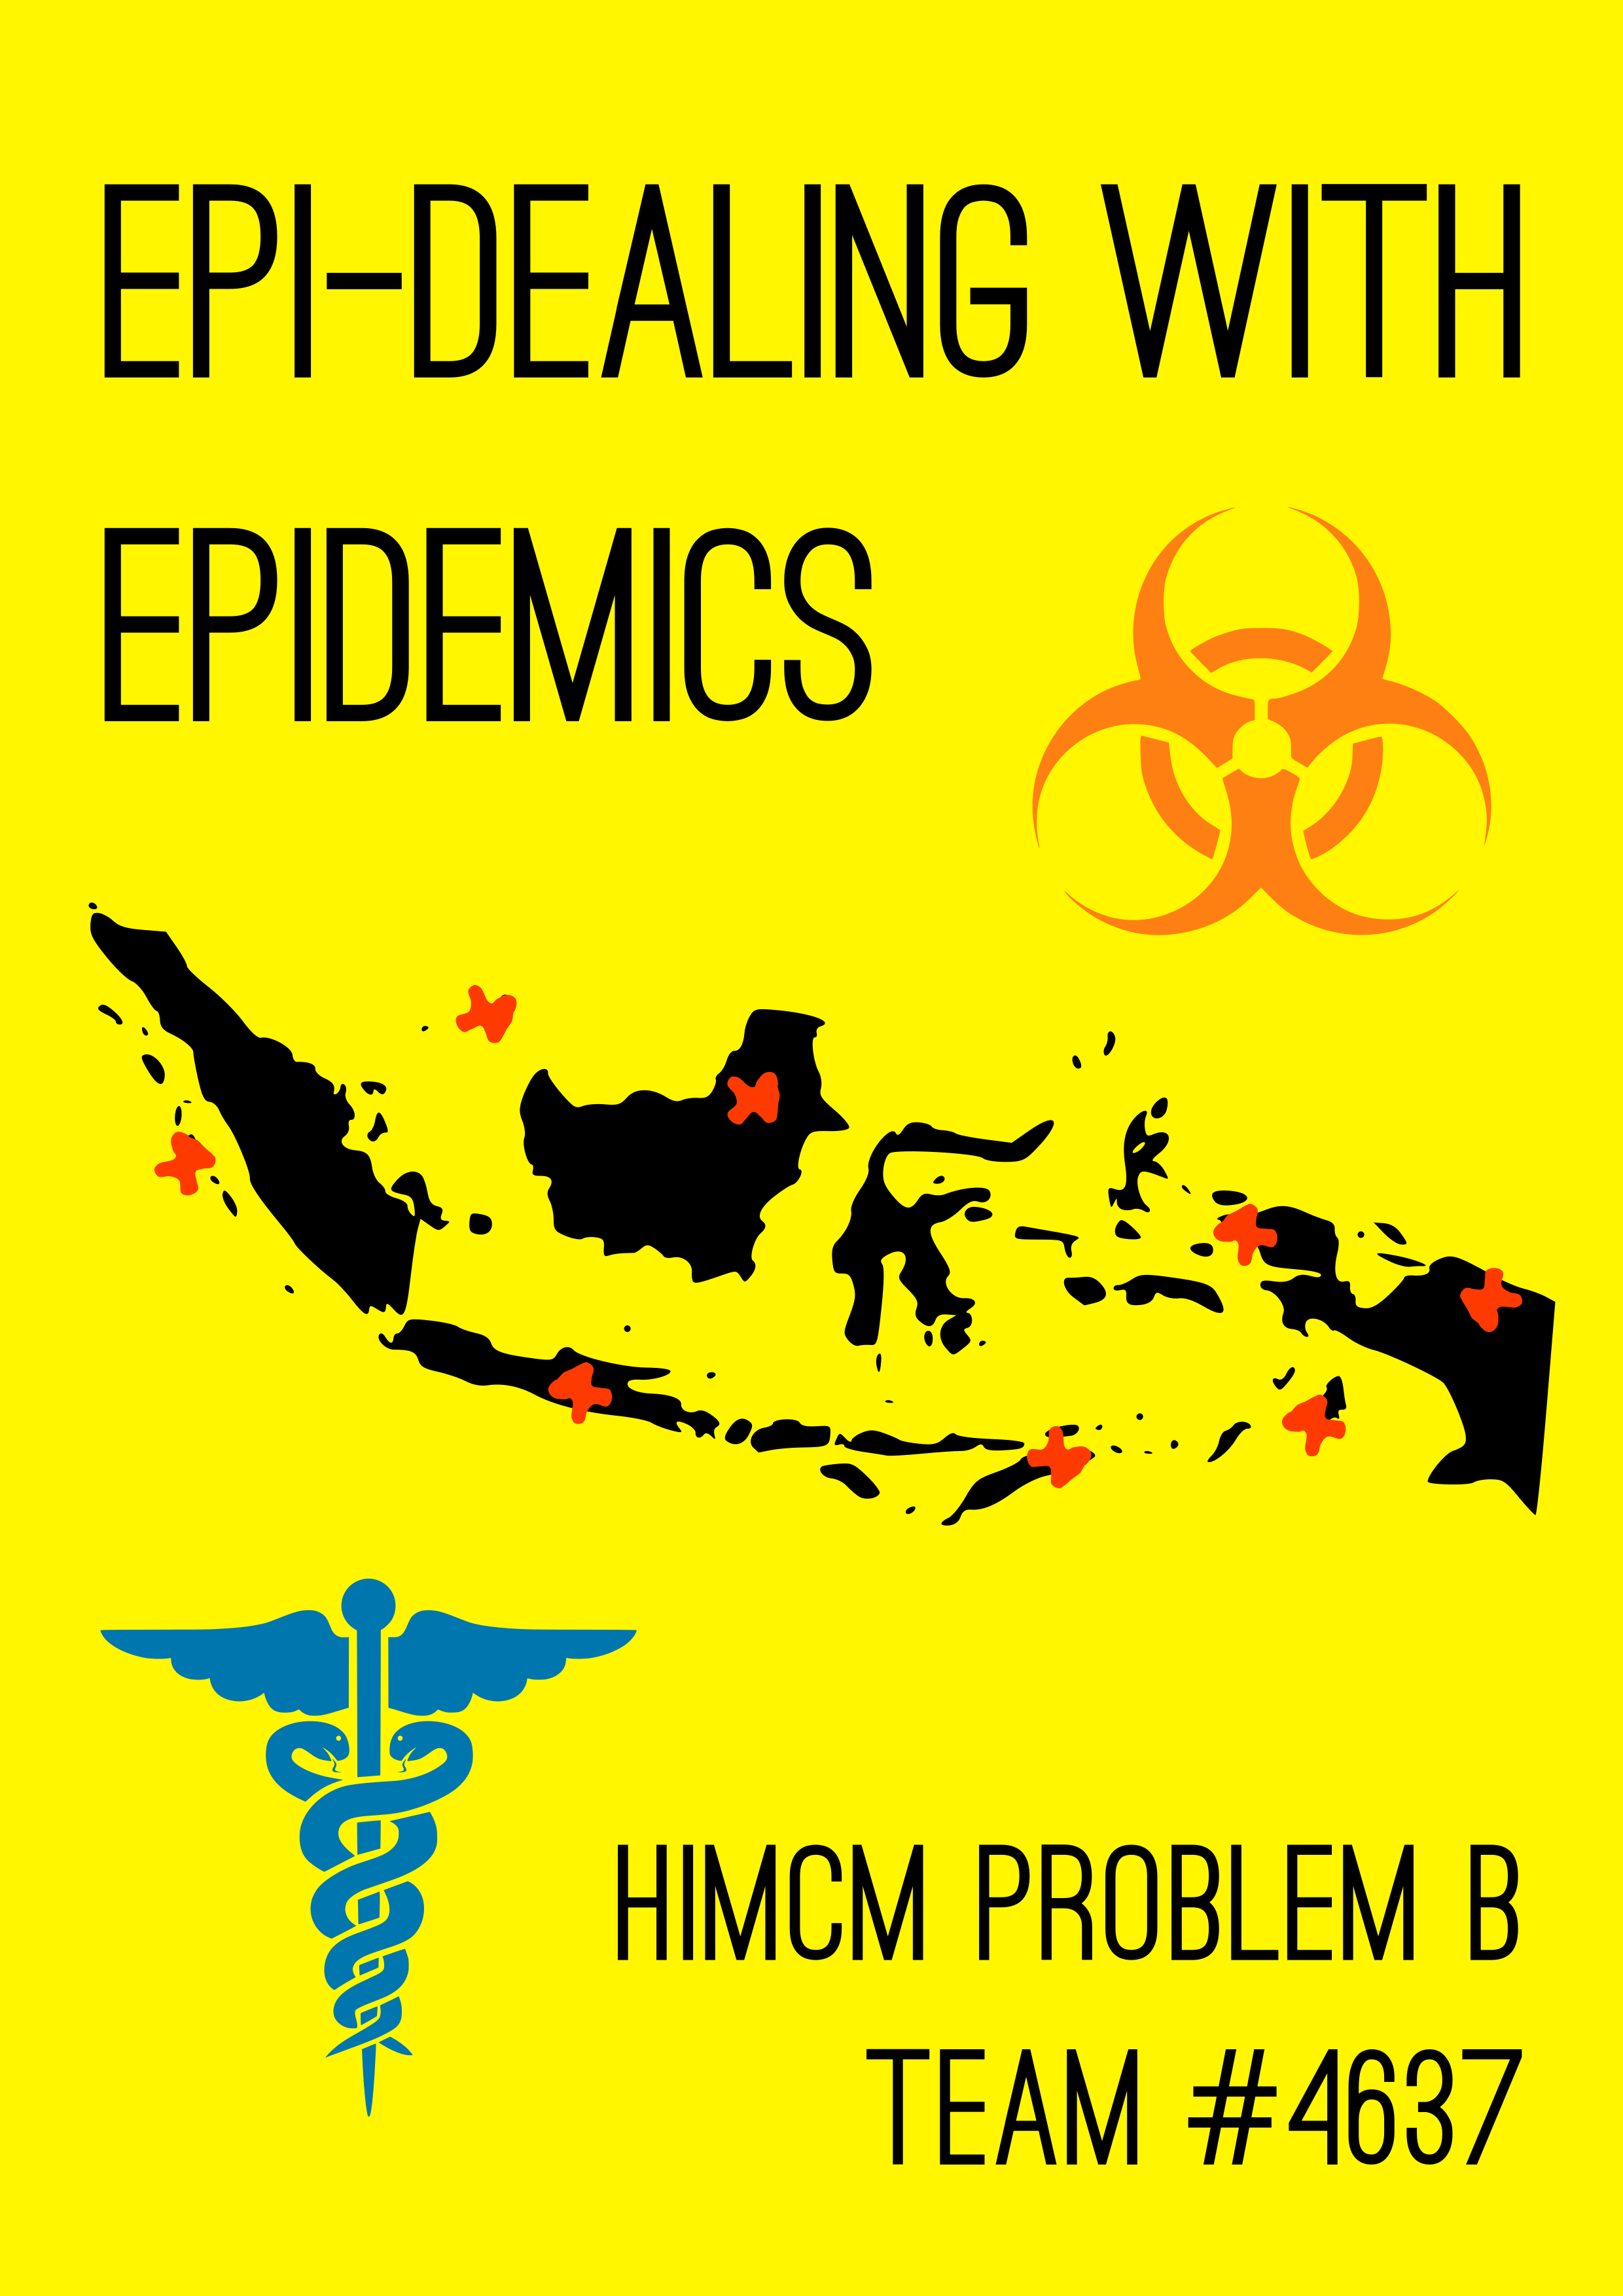
\includegraphics[width=\textwidth]{himcmcover}
\end{center}

\tableofcontents

\newpage
\section{Introduction}
When the infectious Ebola virus reared its ugly head in Africa in the summer of 2014, many people were terrified. How could this virus, previously a seemingly unknown and non-existent threat to humans, cause such devastation in such a short amount of time in many parts of West Africa? In just 6 short months, more than 13,500 cases have been reported, and 4951 humans have perished from this deadly disease. This catastrophe not only devastated and terrified the public, but just as importantly, it also warned them about the necessity of proper disease control methods to prevent a similar tragedy from repeating itself. In addition, it demonstrated the potential damage that a scarcity of proper medical resources, such as doctors, containment centers, money, and drugs, can cause in developing countries, where medical care is not ubiquitous. Therefore, when a strange, unknown disease began to pop up in an isolated village in Indonesia, an ominous parallel between this potential threat and that in West Africa seemed strikingly clear. In this problem, we are tasked with analyzing this potential epidemic in Indonesia, creating a mathematical model to understand the behavior of the disease, as well as determining how to contain it to the best of our ability. Much like the events in West Africa, we are faced with the challenge of limited resources and what ostensibly is a very deadly disease. However, in our case, we will do whatever we can to ensure the tragedy of Ebola does not repeat itself.

What is the background of this novel disease in Indonesia? It was first discovered by a humanitarian mission to the village in question. When they arrived, they found out that 15 people infected by the disease had died in the week before they came, leaving 300 in the village. Slightly less than half of the village’s current inhabitants are showing symptoms of this disease, while the rest--slightly more than half--are not. It is possible that the disease in its current form is a mutation of a similar disease that afflicts a native Indonesian animal. Many similar diseases, which just popped up and previously unknown to be infectious to humans, descend from an animal counterpart. For example, a type of chimpanzee in West Africa was the original source of HIV infection in humans; the counterpart SIV (Simian Immunodeficiency Virus) was before known to affect chimpanzees only. In addition, the previously mentioned Ebola virus is also known to have spread to humans from a monkey infected with a similar disease.

We are faced with the challenge of controlling this unfamiliar disease. To do so, we will first make a mathematical model simulating the disease spread within the village in order to gain a better understanding of this disease, including its potential spread, infectiousness, and classification of spread. In addition, we will determine whether or not this disease can be classified as a contained epidemic. According to WebMD, an epidemic is defined as when an infectious disease spreads rapidly to many people. An epidemic is uncontained when the number of infectious people is increasing, and decreasing when it’s not. Next, we face the task of allocating scarce resources to combat and control the disease, including preventing it from spreading and treating already infected inhabitants. We have limited amounts of resources, including doctors, containment facilities, money, research, and serums, to combat this disease, which is now being monitored by our employer, the International World Health Organization. Our goal is to develop a model that accomplishes all of these tasks.

From the findings of our model, as well as research and observations, we will need to give recommendations on the best course of action to national Centers of Disease Control in order to prevent the spread of this disease. At some point, we expect to receive information from an international research team that will be studying this disease first hand, which we can use to further improve our model. Based on their direct observations, they will be able to provide us with more specific information about the behavior of the disease. In addition, it is possible that that they may be able to give us more information upon our request. After completing our research, we will debrief news outlets around the world on the state of crucial matter, and educate the public about the best practices to help stem the spread of this disease.

\newpage
\section{Assumptions}

\textbf{PRANAV SIVAKUMAR IS A HUGE FAGGOT}

\textbf{Assumption 1:} All symptoms are caused by one disease. An individual who is showing these symptoms has the disease.
\newline
\textbf{Justification:} --removed--

We will also assume that any individual who shows these symptoms has the disease. As we mentioned earlier, no other disease would cause these symptoms. In addition, the problem implies that the symptoms of the disease are noticeable, an uninfected individual will also not display these symptoms. Thus, an individual will have to be infected in order to display these symptoms.
\newline
\newline
\textbf{Assumption 2:} The disease in question is deadly/scary enough that any logical person will avoid being infected by taking preventative precautionary measures.
\newline
\textbf{Justification:} Due to the fact that almost half of the village is infected, and 15 have died, it is reasonable to assume that people regard this disease with apprehension. In addition, since the International World Health Organization and major authorities are involved, word about the danger of this disease will have spread to neighboring villages and islands. Due to this, uninfected people will have less interaction with infected people showing symptoms. In addition, it will be less likely that neighboring villages will accept a stranger showing symptoms into their village.
\newline
\newline
\textbf{Assumption 3:} The village has a constant population for the duration of disease. No people are born or die from causes other than the disease during the course of the disease.
\newline
\textbf{Justification:} A remote Indonesian village will not have very much interaction with the outside world in the first place, barring nearby villages. However, after the village is discovered as having a dangerous infectious disease, there will be extremely minimal interaction between the village and nearby villages or islands, as people will be highly discouraged from entering or leaving the village. It is highly unlikely that a person would enter a village afflicted by a dangerous disease. In addition, people inside the afflicted village will have difficulty leaving; as half the village is infected, they cannot help transport others to nearby villages/islands, not to mention that the authorities of other villages/islands will not allow people from the afflicted village to enter to prevent spread of the disease.

Since this is a potent disease because a near majority of the village is infected, and 15 people were killed in the last week, it is extremely more likely that the disease will kill a given person rather than other causes such as old age. In addition, it’s just as unlikely for new births to occur during this time, as previously mentioned, because many people are currently sick and displaying symptoms.
\newline
\newline
\textbf{Assumption 4:} Rates of transmission from Susceptible to Infected and Infected to Recovered are relatively constant.
\newline
\textbf{Justification:} No information is given that would suggest that rates of transmission change or fluctuate over time. In addition, many other diseases have relatively constant rates of transmission, allowing people to create accurate mathematical models of them. Therefore, we will assume that this disease behaves in a similar manner.
\newline
\newline
\textbf{Assumption 5:} The demographic of the villages in question is representative but not necessarily proportional to the demographic of Indonesia as a whole.
\newline
\textbf{Justification:} Due to lack of information, we cannot directly determine the demographics of the village, so utilizing the country’s whole demographic is the most accurate statistic we can use estimate this demographic. We do need to take into account the demographic of the village in our model, because it affects interactions between people as well as degrees of susceptibility.
\newline
\newline
\textbf{Assumption 6:} The area of the village mirrors the average population density of Indonesia as a whole.
\newline
\textbf{Justification:} The area of the village is an unknown but necessary variable to consider in our model. Thus, basing the area off Indonesia as a whole will result in the most accurate and reasonable assumption of the value of this variable.
\newline
\newline
\textbf{Assumption 7:} Disease is spread through human interaction rather than a vector.
\newline
\textbf{Justification:} Diseases that incorporate vector-based transmission tend to be slower than those that are transmitted through human interaction. The fact that nearly 50\% of the population is infected indicates that this is a disease that spreads quickly -- certainly too quickly for it to be a vector-based disease. In addition, there is no information given whatsoever that justifies a vector-based transmission model.

\newpage
\section{Model}

\subsection{Model I - Standard Condition}

\subsubsection{Goals of Model}

This model was designed to address the following concerns:
\begin{itemize}
	\item Classify the type and severity of an epidemic that is taking place in a small village in Indonesia
	\item Determine if an epidemic is contained or not based on the set of limited information provided and what could be assumed
	\item Distribute various limited sources of aid to contain the disease most efficiently and effectively
	\item Simulate the effect of the disease under different circumstances through repeated run-throughs of the model under different conditions.
\end{itemize}

\subsubsection{Summary of Model Program}

We wrote a program that modelled the spread of the disease through the starting population of the village as described in the problem. Many factors, including transmissibility, avoidance, etc. were unknown but taken into consideration, and will be discussed further later in the paper. We created a village with 300 inhabitants, slightly less of whom were infected with the disease and the rest were healthy but susceptible. We calculated the rates of interaction between infected and healthy people every day to model the transmission of this disease. The program would continue to run until the number of total infected people reached zero. This program was run hundreds of times, under many different starting values of our unknowns, to observe overall trends as well as optimal responses. The full code, written in Java, can be found in the Appendix.

\subsubsection{SIR Model Influences}

The foundation of our models comes from the SIR model, used widely in epidemiology. The SIR model groups people into categories by their relationship with the infectious disease. S stands for susceptible, which is a person who is able to contract the disease. I stands for infected, which is the number of people who currently have the disease. A variation is the SEIR model, which includes Exposed (E), those who have the disease but are in a latent period and do not show any symptoms. For simplicity, we grouped E with I: after catching the disease, a given person would have an incubation period of a non-negative number of days, after which they would start displaying symptoms; however, we considered both of these people as “infected”. Infected people can go in one of two directions. If they recover from the disease, they go into group R, which stands for Recovered. These people gain immunity to the disease and will survive after the infection leaves their body. The rest of the infected people will eventually die as a direct result of the disease.

The SIR model is useful because it allows us to calculate rates of change for each of these categories. From this, we can determine how the infection is moving by seeing the movement of people between categories. Define S, I, and R as the number of people in each of these categories, and N the total number of people. Also, s, i, and r are the ratios of people in each of these categories; \(s=S/N\), \(i=I/N\), and \(r=R/N\). We also define \(\beta = r·c\), where r is the transmissibility, or the probability that an infected person will infect a susceptible person in a given interaction, and c is the average rate of contact between susceptible and infected individuals. Then, we have 𝑑𝑠/𝑑𝑡= = −𝛽𝑠𝑖, 𝑑𝑖/𝑑𝑡 = 𝛽𝑠𝑖−𝑣𝑖, and 𝑑𝑟/𝑑𝑡 = 𝑣𝑖, as illustrated in Figure 1. We know that an uncontained epidemic occurs when the number of infectious cases is increasing, so we must have 𝛽𝑠𝑖 − 𝜈𝑖 > 0 for this to be the case.

\subsection{Implications of Model}

\begin{center}
\[
P=1-\bigg(1-\Big(\frac{\frac{2.5}{Area}*i*(K-\frac{K^2}{N})}{S}\Big)\bigg)^\frac{1}{K}
\]


\begin{tabular}{c || c | c}
\hline
Paul & Jason & Noor \\
\hline
How & Do & You \\
\hline
Like & This & LaTeX \\
\hline
\end{tabular}

\end{center}


\end{document}